\chapter{Dev C++ 的使用}

\section{快捷键}

\begin{table}[h]
  \centering
  \caption{Dev C++ 快捷键一览}
  \begin{tabular}{llll}
    \toprule
    快捷键 & 功能 & 快捷键 & 功能 \\
    \midrule
    Ctrl+N & 新建源代码 & Ctrl+O & 打开文件 \\
    Ctrl+F9 & 编译程序 & Ctrl+F10 & 运行 \\
    F9 & 编译并运行 & F8 & 调试程序 \\
    Ctrl+W & 查看变量 & Ctrl+Alt+F2 & 终止程序 \\
    Ctrl+. & 注释 & Ctrl+M & 取消注释 \\
    Ctrl+Shift+A & 格式化代码 & Ctrl+Space & 代码提示 \\
    \bottomrule
  \end{tabular}
\end{table}

\section{调试}

\begin{figure}[h]
  \centering
  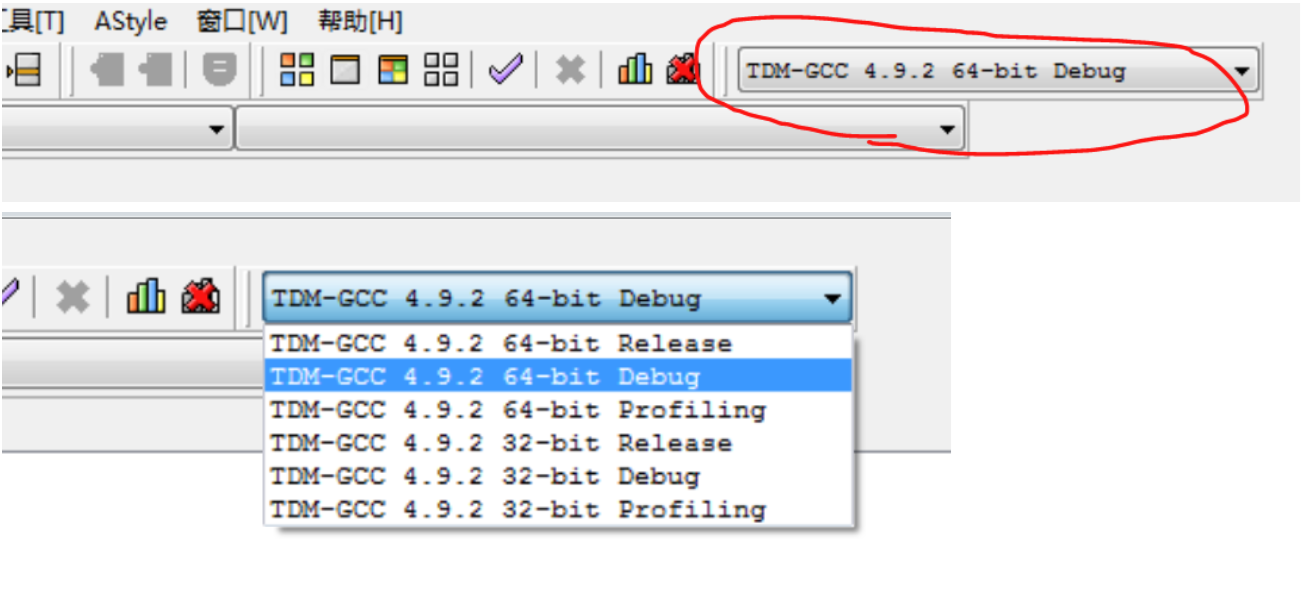
\includegraphics[width=0.70\textwidth]{assets/devcpp_debug.png}
  \caption{打开调试功能}
\end{figure}

先打开调试功能。在行号处点击，这一行会变红，断点就设置在这里；再点击调试按钮，页面会出现黑色的运行框，同时红色断点行变蓝。

输入数据有两种方法：

\begin{enumerate}
  \item 先单步到 \texttt{scanf} 之后，再到运行框输入数据并回车。
  \item 先在运行框输入（输入时不会回显），回车后回到代码框单步，输入内容才会显示。
\end{enumerate}

\section{C++ 标准设置}

\begin{figure}[h]
  \centering
  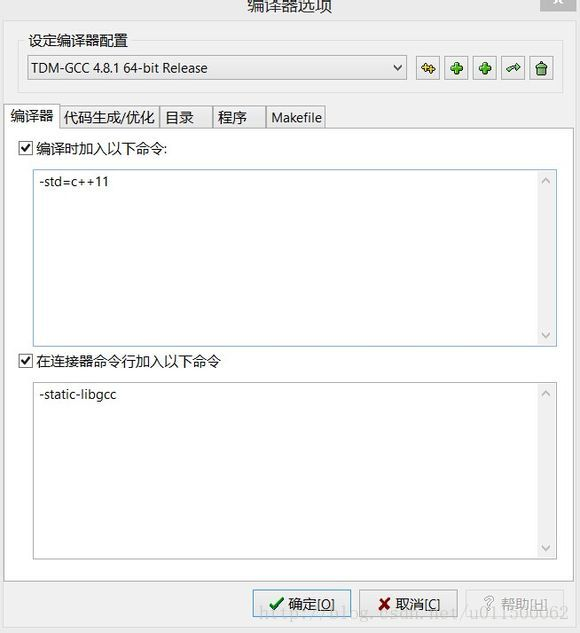
\includegraphics[width=0.70\textwidth]{assets/devcpp_standard.jpg}
  \caption{调整编译标准}
\end{figure}

\begin{enumerate}
  \item 在 Dev 的【工具】里找到【编译选项】。
  \item 【编译时加入以下命令】原本是空白且未勾选；勾选后填入 \texttt{-std=c++17}（旧版本可填 \texttt{-std=c++11}）。
\end{enumerate}

\section{优化开关}

O1 主要优化分支、常量与表达式；O2 在此基础上做更多寄存器级与指令级优化，编译更慢；O3 在 O2 上继续增加内联与循环优化。

\begin{codeline}
#pragma GCC optimize(2)
#pragma GCC optimize(3,"Ofast","inline")
\end{codeline}
